\iffalse
\title{2013-ME-13-24}
\author{EE24Btech11024 - G. Abhimanyu Koushik}
\section{me}
\chapter{2013}
\fi

\item The function $f\brak{t}$ satisfies the differential equation $\frac{d^2f}{dt^2}+f=0$ and the auxillary conditions, $f\brak{0}=0$, $\frac{df}{dt}\brak{0}=4$. The Laplace transform of $f\brak{t}$ is given by

	\hfill{\brak{\text{ME 2013}}}
	\begin{multicols}{4}
		\begin{enumerate}
			\item $\frac{2}{s+1}$
			\item $\frac{4}{s+1}$
			\item $\frac{4}{s^2+1}$
			\item $\frac{2}{s^4+1}$
		\end{enumerate}
	\end{multicols}

\item Specific enthalpy and velocity of steam at inlet and exit of a steam turbine, running under steady state, are as given below:
	\\\begin{table}[h!]    
		\centering
		\resizebox{0.7\textwidth}{!}{{\begin{tabular}[12pt]{|c|c|c|}
			\hline
			& Specific enthalpy \brak{kJ/kg} & Velocity \brak{m/s} \\
			\hline
			Inlet steam condition & $3250$ & $180$ \\
			\hline
			Exit steam condition & $2360$ & $5$ \\
			\hline
		\end{tabular}
		}}
	\end{table}\\
	The rate of heat loss from the turbine per $kg$ of steam flow rate is $5$ $kW$. Neglecting changes in potential energy of steam, the power developed in $kW$ by the steam turbine per $kg$ of the steam flow rate is

	\hfill{\brak{\text{ME 2013}}}
	\begin{enumerate}
			\begin{multicols}{4}
			\item $901.2$
			\item $911.2$
			\item $17072.5$
			\item $17082.5$
			\end{multicols}
	\end{enumerate}

\item A steel ball of diameter $60$ $mm$ is initially in thermal equilibrium at $1030^{\degree} C$ in a furnace. It is suddenly removed from the furnace and cooled in ambient air at $30^{\degree} C$, with convective heat transfer coefficient $h=20$ $W/m^2K$. The thermo-physical properties of steel are: density $\rho=7800$ $kg/m^3$, conductivity $k=40$ $W/mK$ and specific heat $c=600$ $J/kgK$. The time required in seconds to cool the steel ball in air from $1030^{\degree} C$ to $430^{\degree} C$ is

	\hfill{\brak{\text{ME 2013}}}
	\begin{enumerate}
			\begin{multicols}{4}
			\item $519$
			\item $931$
			\item $1195$
			\item $2144$
			\end{multicols}
	\end{enumerate}

\item A flywheel is connected to a punching machine has a supply energy of $400$ $Nm$ while running at mean angular speed of $20$ $rad/s$. If the total fluctuation of speed is not to exceed $\pm 2\%$, the mass moment inertia of the flywheel in $kg-m^2$ is

	\hfill{\brak{\text{ME 2013}}}
	\begin{enumerate}
			\begin{multicols}{4}
			\item $25$
			\item $50$
			\item $100$
			\item $125$
			\end{multicols}
	\end{enumerate}

\item A compound gear train with gears $P$, $Q$, $R$ and $S$ has number of teeth $20$, $40$, $15$ and $20$, respectively. Gears $Q$ and $R$ are mounted on the same shaft as shown in the figure below. The diameter of the gear $Q$ is twice that of the gear $R$. If the module of the gear $R$ is $2$ $mm$, the centre distance in $mm$ between the gears $P$ and $S$ is
	\\\begin{center}
		\scalebox{0.5}{
			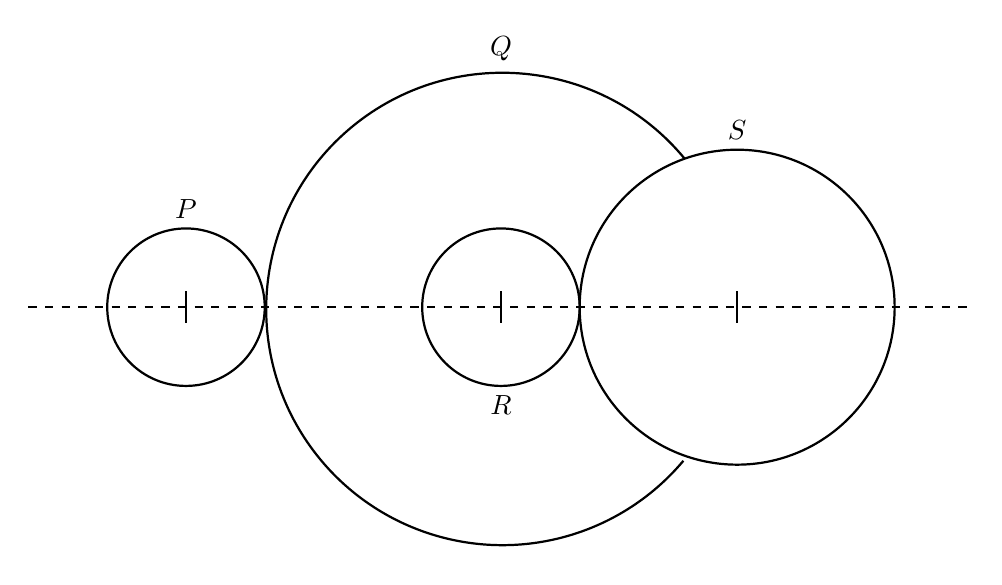
\begin{tikzpicture}
				\draw[draw=black, semithick, dashed] (-6,0) -- (6,0);
				\draw[draw=black, thick, solid] (-4,0) circle (1.00);
				\draw[draw=black, thick, solid] (2.333334,1.88563) arc[start angle=39.5, end angle=320, radius=3];
				\draw[draw=black, thick, solid] (0,0) circle (1.00);
				\draw[draw=black, thick, solid] (3,0) circle (2);

				\draw[draw=black, thick, solid] (-4,0.2) -- (-4,-0.2);
				\draw[draw=black, thick, solid] (0,0.2) -- (0,-0.2);
				\draw[draw=black, thick, solid] (3,0.2) -- (3,-0.2);

				\draw[] (-4,1) node[above] {$P$};
				\draw[] (0,-1) node[below] {$R$};
				\draw[] (0,3) node[above] {$Q$};
				\draw[] (3,2) node[above] {$S$};
			\end{tikzpicture}}
	\end{center}

	\hfill{\brak{\text{ME 2013}}}
	\begin{enumerate}
			\begin{multicols}{4}
			\item $40$
			\item $80$
			\item $120$
			\item $160$
			\end{multicols}
	\end{enumerate}

\item A pin jointed uniform rigid rod of weight $W$ and length $L$ is supported horizontally by an external force $F$ as shown in the figure below. The force $F$ is suddenly removed. At the instant of force removal, the magnitude of vertical reaction developed at the support is
\\\begin{center}
   \scalebox{0.5}{\usetikzlibrary{patterns}
\begin{tikzpicture}
\tikzstyle{every node}=[font=\LARGE]
	\draw [line width=0.8pt] (6.25,15.5) circle (0.25cm);
	\draw [line width=4pt] (6.5,15.5) -- (16.25,15.5);
	\draw[] (5,14.75) rectangle (7.5,14.25);
	\draw [line width=0.8pt, ->, >=Stealth] (16.25,13) -- (16.25,15.5);
	\draw [line width=0.8pt, ->, >=Stealth] (11.25,11.75) -- (6.25,11.75);
	\draw [line width=0.8pt, ->, >=Stealth] (11.25,11.75) -- (16.25,11.75);
	\draw[] (16.25,14.25) node[right] {$F$};
	\draw[] (11.25,12.25) node[above] {$L$};
	\draw [line width=0.8pt] (16.25,11.25) -- (16.25,12.25);
	\draw [line width=0.8pt] (6.25,11.25) -- (6.25,12.25);
	\draw [line width=0.8pt] (5,14.75) -- (7.5,14.75);
	\draw [line width=0.8pt] (5.75,15.5) -- (5.75,14.75);
	\draw [line width=0.8pt] (6.75,15.5) -- (6.75,14.75);
	\draw [line width=0.8pt] (6.75,15.5) arc[start angle=0, end angle=180, radius=0.5cm];
\end{tikzpicture}}
\end{center}

	\hfill{\brak{\text{ME 2013}}}
	\begin{enumerate}
			\begin{multicols}{4}
			\item zero
			\item $\frac{W}{4}$
			\item $\frac{W}{2}$
			\item $W$
			\end{multicols}
	\end{enumerate}

\item Two cutting tools are being compared for a machine operation. The tool life equations are:
	\\\begin{table}[h!]    
		\centering
		\resizebox{0.3\textwidth}{!}{\begin{tabular}{rl}
			Carbide tool: & $VT^{1.6}=3000$ \\
			HSS tool: & $VT^{0.6}=200$ \\
		\end{tabular}}
	\end{table}\\
	where $V$ is the cutting speed in $m/min$ and T is the tool life in $min$. The carbide tool will provide higher tool life if the cutting speed in $m/min$ exceeds 

	\hfill{\brak{\text{ME 2013}}}
	\begin{enumerate}
			\begin{multicols}{4}
			\item $15.0$
			\item $39.4$
			\item $49.3$
			\item $60.0$
			\end{multicols}
	\end{enumerate}

\item In a CAD package, mirror image of a 2D point $\vec{P}\brak{5,10}$ is to be obtained about a line which passes through origin and makes an angle $45^{{{{{\degree}}}}}$ counterclockwise with the X-axis. The coordinates of transformed point will be

	\hfill{\brak{\text{ME 2013}}}
	\begin{enumerate}
			\begin{multicols}{4}
			\item $\brak{7.5,5}$
			\item $\brak{10,5}$
			\item $\brak{7.5,-5}$
			\item $\brak{10,-5}$
			\end{multicols}
	\end{enumerate}

\item A linear programming problem is shown below.
	\\\begin{table}[h!]    
		\centering
		\resizebox{0.3\textwidth}{!}{\begin{tabular}{rl}
			Maximize & $3x + 7y$ \\[10pt]
			Subject to & $3x + 7y \leq 10$ \\
			& $4x + 6y \leq 8$ \\
			& $x, y \geq 0$
		\end{tabular}}
	\end{table}\\
	It has

	\hfill{\brak{\text{ME 2013}}}
	\begin{enumerate}
			\begin{multicols}{2}
			\item an unbounded objective function.
			\item exactly one optimal solution.
			\item exactly two optimal solutions.
			\item infinitely many optimal solutions.
			\end{multicols}
	\end{enumerate}

\item Cylindrical pins of $25^{\substack{+0.020\\+0.010}}$ $mm$ diameter are electroplated in a shop. Thickness of the plate is $30^{\pm 2.0}$ $micron$. Neglecting gauge tolerances, the size of the GO gauge in $mm$ to inspect the plated components is 

	\hfill{\brak{\text{ME 2013}}}
	\begin{enumerate}
			\begin{multicols}{4}
			\item $25.042$
			\item $25.052$
			\item $25.074$
			\item $25.084$
			\end{multicols}
	\end{enumerate}

\item During the electrochemical machining \brak{\text{ECM}} of iron \brak{\text{atomic weight}=56\text{, valency}=2} at current $1000$ $A$ with $90\%$ current efficiency, the material removal rate was observed to be $0.26$ $gm/s$. If the Titanium \brak{\text{atomic weight}=48\text{, valency}=3} is machined by ECM process at the current of $2000$ $A$ with $90\%$ current efficiency, the expected material removal rate in $gm/s$ will be

	\hfill{\brak{\text{ME 2013}}}
	\begin{enumerate}
			\begin{multicols}{4}
			\item $0.11$
			\item $0.23$
			\item $0.30$
			\item $0.52$
			\end{multicols}
	\end{enumerate}

\item A single degree of freedom system having mass $1$ $kg$ and stiffness $10$ $kN/m$ initially at rest is subjected to an impulse force of magnitude $5$ $kN$ for $10^{-4}$ $seconds$. The amplitude in $mm$ if the resulting free vibration is

	\hfill{\brak{\text{ME 2013}}}
	\begin{enumerate}
			\begin{multicols}{4}
			\item $0.5$
			\item $1.0$
			\item $5.0$
			\item $10.0$
			\end{multicols}
	\end{enumerate}

